\let\negmedspace\undefined
\let\negthickspace\undefined
\documentclass[journal]{IEEEtran}
\usepackage[a5paper, margin=10mm, onecolumn]{geometry}
\usepackage{lmodern} % Ensure lmodern is loaded for pdflatex
\usepackage{tfrupee} % Include tfrupee package

\setlength{\headheight}{1cm} % Set the height of the header box
\setlength{\headsep}{0mm}     % Set the distance between the header box and the top of the text

\usepackage{gvv-book}
\usepackage{gvv}
\usepackage{cite}
\usepackage{amsmath,amssymb,amsfonts,amsthm}
\usepackage{algorithmic}
\usepackage{graphicx}
\usepackage{textcomp}
\usepackage{xcolor}
\usepackage{txfonts}
\usepackage{listings}
\usepackage{enumitem}
\usepackage{mathtools}
\usepackage{gensymb}
\usepackage{comment}
\usepackage[breaklinks=true]{hyperref}
\usepackage{tkz-euclide} 
\usepackage{listings}
\usepackage{gvv}                                        
\def\inputGnumericTable{}                                 
\usepackage[latin1]{inputenc}                                
\usepackage{color}                                            
\usepackage{array}                                            
\usepackage{longtable}                                       
\usepackage{calc}                                             
\usepackage{multirow}                                         
\usepackage{hhline}                                           
\usepackage{ifthen}                                           
\usepackage{lscape}

\bibliographystyle{IEEEtran}
\vspace{3cm}

\title{8.2.2}
\author{EE24BTECH11004 - Ankit Jainar}
\date{}

\begin{document}

\bibliographystyle{IEEEtran}
\vspace{3cm}

\maketitle

\bigskip

\textbf{Question:}
Find the area bounded by the curves:
\begin{align}
    (x - 1)^2 + y^2 = 1 \quad \text{and} \quad x^2 + y^2 = 1
\end{align}
\newline

\textbf{Theoretical Solution:}

The curves are two circles:
\begin{itemize}
    \item Circle 1: $(x - 1)^2 + y^2 = 1$, centered at $(1, 0)$ with radius $1$.
    \item Circle 2: $x^2 + y^2 = 1$, centered at $(0, 0)$ with radius $1$.
\end{itemize}

\textbf{Step 1: Finding the Points of Intersection Using Theoritical Approach}

The points of intersection occur where the two circles overlap. To find the intersection points, we rewrite the equations as:
\begin{align}
    (x - 1)^2 + y^2 &= 1 \quad \text{(Circle 1)} \\
    x^2 + y^2 &= 1 \quad \text{(Circle 2)}
\end{align}

Expanding both equations:
\begin{align}
    x^2 - 2x + 1 + y^2 &= 1 \quad \text{(Circle 1)} \\
    x^2 + y^2 &= 1 \quad \text{(Circle 2)}
\end{align}

Subtracting the second equation from the first gives:
\begin{align}
    -2x + 1 &= 0 \quad \implies \quad x = \frac{1}{2}
\end{align}

Substituting $x = \frac{1}{2}$ into the equation of Circle 2:
\begin{align}
    \left(\frac{1}{2}\right)^2 + y^2 &= 1 \\
    \frac{1}{4} + y^2 &= 1 \\
    y^2 &= \frac{3}{4} \quad \implies \quad y = \pm \frac{\sqrt{3}}{2}
\end{align}

Thus, the points of intersection are:
\begin{align}
    P_1 = \left(\frac{1}{2}, \frac{\sqrt{3}}{2}\right), \quad P_2 = \left(\frac{1}{2}, -\frac{\sqrt{3}}{2}\right)
\end{align}

Matrix representation for solving this system:
\begin{align}
    \bm{A} \cdot \bm{x} = \bm{b},
\end{align}
where:
\begin{align}
    V_1 &= \begin{pmatrix} 2 & 0 \\ 1 & 1 \end{pmatrix}, \quad
    \vec{x} = \begin{pmatrix} x \\ y^2 \end{pmatrix}, \quad
    \vec{b} = \begin{pmatrix} 1 \\ 1 \end{pmatrix}.
\end{align}

\textbf{Step 2:Intersection of Two Circles Using Matrix Approach}

\textbf{ General Form of the Circle Equations}

The general form for a circle is:
\begin{align}
    g(x, y) &= \vec{x}^\top V \vec{x} + 2 \vec{u}^\top \vec{x} + f = 0
\end{align}

For Circle 1: \( (x - 1)^2 + y^2 = 1 \)
\begin{align}
    g_1(x, y) &= \vec{x}^\top V_1 \vec{x} + 2 \vec{u}_1^\top \vec{x} + f_1 = 0 \\
    V_1 &= \begin{pmatrix} 1 & 0 \\ 0 & 1 \end{pmatrix}, \quad
    \vec{u}_1 = \begin{pmatrix} -1 \\ 0 \end{pmatrix}, \quad
    f_1 = 0
\end{align}

For Circle 2: \( x^2 + y^2 = 1 \)
\begin{align}
    g_2(x, y) &= \vec{x}^\top V_2 \vec{x} + 2 \vec{u}_2^\top \vec{x} + f_2 = 0 \\
    V_2 &= \begin{pmatrix} 1 & 0 \\ 0 & 1 \end{pmatrix}, \quad
    \vec{u}_2 = \begin{pmatrix} 0 \\ 0 \end{pmatrix}, \quad
    f_2 = -1
\end{align}

\textbf{ Subtract the Equations to Eliminate Quadratic Terms}

Subtract \( g_1(x, y) \) from \( g_2(x, y) \):
\begin{align}
    g_2(x, y) - g_1(x, y) &= (\vec{x}^\top V_2 \vec{x} + 2 \vec{u}_2^\top \vec{x} + f_2) - (\vec{x}^\top V_1 \vec{x} + 2 \vec{u}_1^\top \vec{x} + f_1) = 0 \\
    0 &= 2 (\vec{u}_2 - \vec{u}_1)^\top \vec{x} + (f_2 - f_1)
\end{align}

Simplify:
\begin{align}
    2 \begin{pmatrix} 0 - (-1) \\ 0 - 0 \end{pmatrix}^\top \vec{x} + (-1 - 0) = 0 \\
    2 \begin{pmatrix} 1 \\ 0 \end{pmatrix}^\top \vec{x} - 1 = 0
\end{align}

\textbf{ Line Equation Representing the Chord of Intersection}

The line equation representing the chord of intersection is:
\begin{align}
    \begin{pmatrix} 1 \\ 0 \end{pmatrix}^\top \vec{x} = \frac{1}{2}
\end{align}

This simplifies to:
\begin{align}
    x = \frac{1}{2}.
\end{align}

\textbf{ Substituting \( x \) into One Circle Equation}

Substitute \( x = \frac{1}{2} \) into the second circle equation \( g_2(x, y) \):
Substituting \(\vec{x}\) into the circle equation:
\begin{align}
    \begin{pmatrix} \frac{1}{2} \\ y \end{pmatrix}^\top \begin{pmatrix} 1 & 0 \\ 0 & 1 \end{pmatrix} \begin{pmatrix} \frac{1}{2} \\ y \end{pmatrix} - 1 = 0.
\end{align}

Expanding the terms:
\begin{align}
    \frac{1}{4} + y^2 - 1 = 0.
\end{align}

Simplifying:
\begin{align}
    y^2 = \frac{3}{4}.
\end{align}

Thus:
\begin{align}
    y = \pm \frac{\sqrt{3}}{2}.
\end{align}

\textbf{ Points of Intersection}

The points of intersection are:
\begin{align}
    \vec{x}_1 &= \begin{pmatrix} \frac{1}{2} \\ \frac{\sqrt{3}}{2} \end{pmatrix}, \quad
    \vec{x}_2 = \begin{pmatrix} \frac{1}{2} \\ -\frac{\sqrt{3}}{2} \end{pmatrix}.
\end{align}


\textbf{Step 3: Area Calculation Using Trapezoidal Rule}

The area between the two circles is symmetric about the $x$-axis. Therefore, we calculate the area of the upper region and multiply it by $2$.


The area is given by:
\begin{align}
    A = 2 \int_{x=0.5}^{x=1} \left[ \sqrt{1 - (x - 1)^2} - \sqrt{1 - x^2} \right] dx
\end{align}

Expanding $1 - (x - 1)^2$:
\begin{align}
    1 - (x - 1)^2 &= 1 - (x^2 - 2x + 1) \\
    &= 2x - x^2
\end{align}

Thus, the integral becomes:
\begin{align}
    A = 2 \int_{x=0.5}^{x=1} \left[ \sqrt{2x - x^2} - \sqrt{1 - x^2} \right] dx
\end{align}

\textbf{Trapezoidal Rule:}

We discretize the interval $[0.5, 1]$ into $N$ equal subintervals of width $h$:
\begin{align}
    h = \frac{1 - 0.5}{N} = \frac{0.5}{N}.
\end{align}

The $x_k$ values are:
\begin{align}
    x_k = 0.5 + k \cdot h, \quad k = 0, 1, 2, \dots, N.
\end{align}

The area is approximated as:
\begin{align}
    A \approx 2 \cdot h \cdot \left[ \frac{1}{2}(f(x_0) - g(x_0)) + \sum_{k=1}^{N-1} (f(x_k) - g(x_k)) + \frac{1}{2}(f(x_N) - g(x_N)) \right],
\end{align}
where:
\begin{align}
    f(x_k) = \sqrt{2x_k - x_k^2}, \quad g(x_k) = \sqrt{1 - x_k^2}.
\end{align}

\textbf{Difference Equation:}

The iterative formula for the trapezoidal rule is:
\begin{align}
    A_{\text{new}} = A_{\text{old}} + h \cdot \left[(f(x_{k+1}) - g(x_{k+1})) + (f(x_k) - g(x_k)) \right].
\end{align}
\begin{align}
    A_{\text{new}} = A_{\text{old}} + h \cdot \bigg[ & \left(\sqrt{2x_{k+1} - x_{k+1}^2} - \sqrt{1 - x_{k+1}^2}\right) \nonumber \\
    & + \left(\sqrt{2x_k - x_k^2} - \sqrt{1 - x_k^2}\right) \bigg].
\end{align}

The difference equation for the area is given as:
\begin{align}
    A_{n + 1} &= A_n + \frac{h}{2} \left[ y(x_n) + h \cdot y^{\prime}(x_n) + y(x_n) \right] \\
    A_{n + 1} &= A_n + h \cdot \left[ y(x_n) + \frac{h}{2} y^{\prime}(x_n) \right] \\
    A_{n + 1} &= A_n + h \cdot y(x_n) + \frac{h^2}{2} y^{\prime}(x_n)
\end{align}

The curves given are:
\begin{align}
    (x - 1)^2 + y^2 = 1 \quad \text{and} \quad x^2 + y^2 = 1.
\end{align}
Rearranging the equations for \( y(x) \), the piecewise function for the bounded region is:
\begin{align}
    y(x) =
    \begin{cases}
        \sqrt{1 - x^2} & \quad 0 \leq x \leq \frac{1}{2} \\
        \sqrt{1 - (x - 1)^2} & \quad \frac{1}{2} \leq x \leq 1
    \end{cases}
\end{align}

\textbf{Substituting \( y(x) \) into the Difference Equation:}
\newline
By substituting the piecewise function \( y(x) \) into the difference equation, we get:
\begin{align}
    A_{n + 1} &=
    \begin{cases}
        A_n + h \sqrt{1 - x_n^2} + \frac{h^2}{2} \left(-\frac{x_n}{\sqrt{1 - x_n^2}} \right) & \quad 0 \leq x_n \leq \frac{1}{2}, \\
        A_n + h \sqrt{1 - (x_n - 1)^2} + \frac{h^2}{2} \left(-\frac{(x_n - 1)}{\sqrt{1 - (x_n - 1)^2}} \right) & \quad \frac{1}{2} \leq x_n \leq 1.
    \end{cases}
\end{align}

The value of \( x_{n+1} \) is updated as:
\begin{align}
    x_{n+1} = x_n + h.
\end{align}

\textbf{Computational Area:}
\newline
Using the trapezoidal rule with a small step size \( h \), the computational area is: $1.2284$

\textbf{Theoretical Area:}
\newline
Using the analytical approach, the theoretical area is:$\frac{2\pi}{3} - \frac{\sqrt{3}}{2} \approx 1.22837$

By substituting the values of $x_k$, $f(x_k)$, and $g(x_k)$ into the trapezoidal rule, we compute the area iteratively.


\begin{figure}[h!]
    \centering
    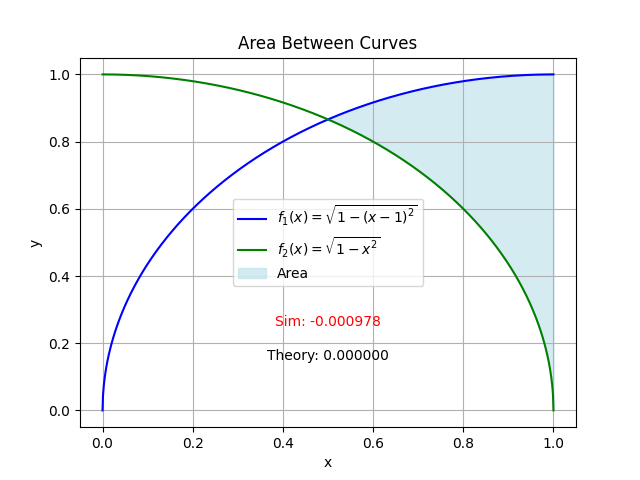
\includegraphics[width=\columnwidth]{figs/fig.png} 
\end{figure}

\end{document}

